%!TEX root =../quadrotorbook.tex

\chapter{Visual Tracking}
\label{chap:tracking}

In this chapter we will introduce algorithms for target tracking and target following.  Target tracking algorithms produce an estimate state of moving targets in the environment, in addition to their uncertainty.  Target following algorithms maneuver the multirotor to follow one of the targets.  The architecture discussed in this chapter is shown in Figure~\ref{fig:tracking_architecture}.
\begin{marginfigure}
	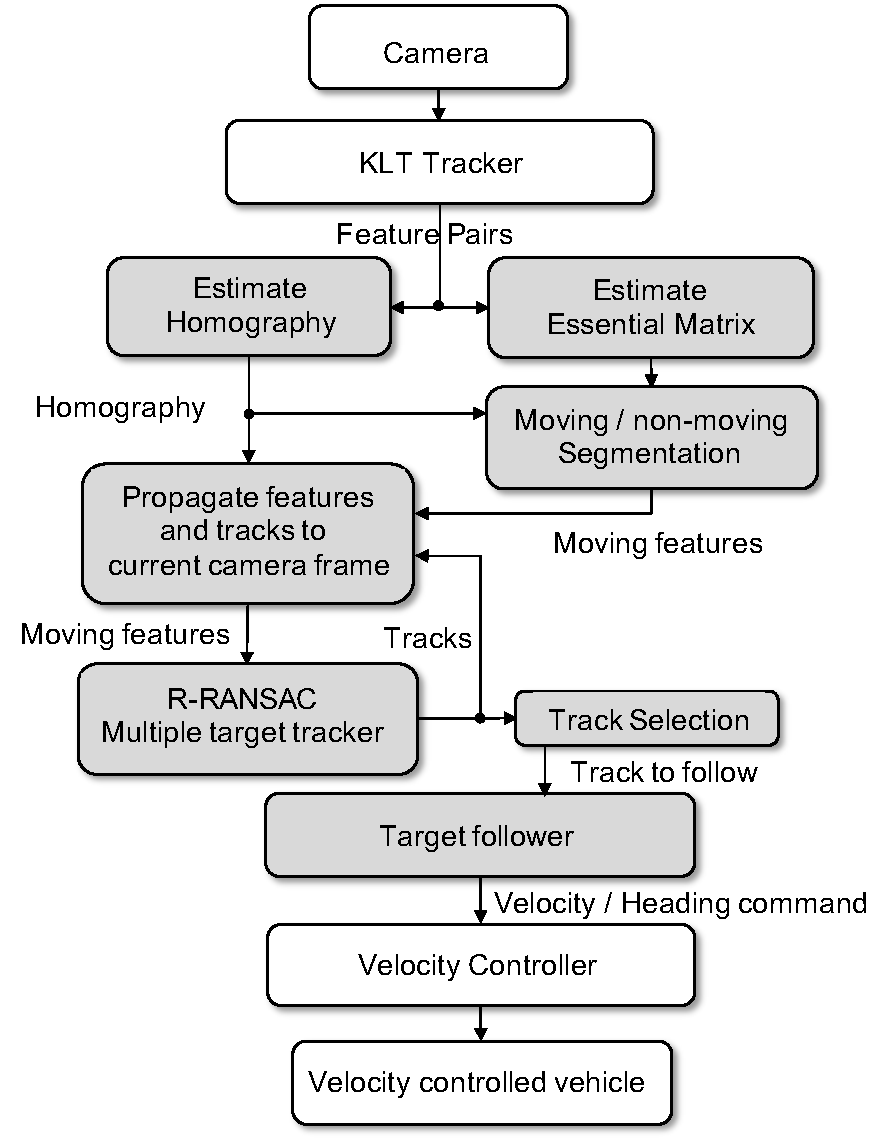
\includegraphics[width=\linewidth]{chap10_tracking/figures/tracking_architecture.pdf} 
	\caption{The architecture for target tracking and following.}
	\label{fig:tracking_architecture}
\end{marginfigure}
As shown in Figure~\ref{fig:tracking_architecture}, the KLT tracker produces a set of feature pairs.  The feature pairs are used to estimate the homography transformation that maps features from the image at time $k-1$ to the image at time $k$.  The feature pairs are also used to estimate the essential matrix between frames.  The homography and essential matrix are used to segment the feature pairs into pairs that move in the image due to the ego-motion of the multi-rotor, and pairs that are actually moving in the scene.  The homography matrix is then used to transform all moving feature pairs, as well all target tracks to the current camera frame.  Moving features are processed by the Recursive-RANSAC multiple target tracker to produce states (position, velocity, acceleration) and covariances of all moving tracks, no the image plane.  The tracks are then processed by a track selection block to select the specific track to follow.  The target follower commands a velocity and heading vector that forces the multirotor to follow the target.  The velocity controller then controls the multirotor to follow that velocity.

Section~\ref{sec:homography_matrix} discusses the homography matrix, and how it can be estimated. Section~\ref{sec:essential_matrix} discusses the essential matrix estimation.
The segmentation algorithm is discussed in Section~\ref{sec:moving_segmentation}, and feature propagation is discussed in Section~\ref{sec:feature_track_propagation}.
Section~\ref{sec:RRANSAC} describes the R-RANSAC tracking algorithm.  Track selection is discussed in Section~\ref{sec:track_selection}, and target following algorithms are described in Section~\ref{sec:target_following}.

%----------------------------------------------------------------------------
\section{The Euclidian homography matrix}
\label{sec:homography_matrix}


This section gives a brief derivation of the Euclidian homography matrix between two camera poses.  The relevant geometry is shown in Figure~\ref{fig:homography_quad}.  
\begin{marginfigure}
	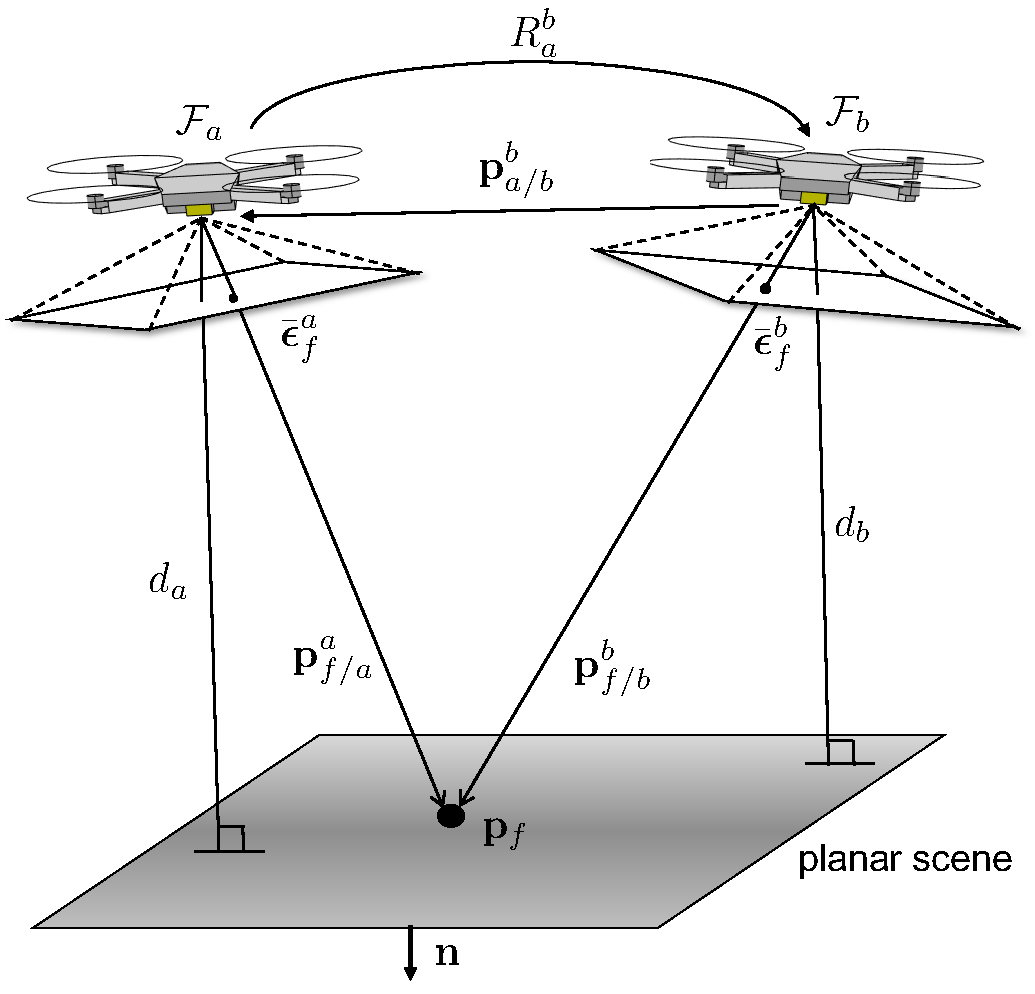
\includegraphics[width=\linewidth]{chap10_tracking/figures/homography_quad.pdf} 
	\caption{The geometry for the derivation of the homography matrix between two camera poses.}
	\label{fig:homography_quad}
\end{marginfigure}
Suppose that $\pbf_f$ is a feature point that lies on a plane defined by the normal (unit) vector $\nbf$.  Let $\pbf_{f/a}^a$ and $\pbf_{f/b}^b$ be the position of $\pbf_f$ relative to frames $a$ and $b$, expressed in those frames respectively. Then as shown in Figure~\ref{fig:homography_quad} we have
\[
\pbf_{f/b}^b = R_a^b \pbf_{f/a}^a + \pbf_{a/b}^b,
\]
where $R_a^b$ is the rotation matrix from frame $a$ to frame $b$, and $\pbf_{a/b}^b$ is the position of frame $a$ relative to frame $b$ expressed in frame $b$.

Let $d_a$ be the distance from the origin of frame $a$ to the planar scene, and observe that
\[
d_a = \nbf^\top \pbf_{f/a}^a \qquad \implies \qquad \frac{\nbf^\top \pbf_{f/a}^a}{d_a} = 1.
\]
Therefore, we get that
\begin{align}
\pbf_{f/b}^b &= R_a^b \pbf_{f/a}^a + \pbf_{a/b}^b \notag \\
			 &= R_a^b \pbf_{f/a}^a + \pbf_{a/b}^b\left(\frac{\nbf^\top \pbf_{f/a}^a}{d_a}\right) \notag \\
			 &= \left(R_a^b  + \frac{\pbf_{a/b}^b}{d_a}\nbf^\top \right) \pbf_{f/a}^a.
			 \label{eq:homography_transformation_1}
\end{align}
Let $\pbf_{f/a}^a = (p_{xa}, p_{ya}, p_{za})^\top$ and $\pbf_{f/b}^b = (p_{xb}, p_{yb}, p_{zb})^\top$, and let $\bar{\epsilonbf}^a = (p_{xa}/p_{za}, p_{ya}/p_{za}, 1)^\top$ represent the normalized homogeneous coordinates of $\pbf_{f/a}^a$ projected onto image plane $a$, and similarly for $\bar{\epsilonbf}^b$.  Then Equation~\eqref{eq:homography_transformation_1} can be written as
\begin{equation}\label{eq:homography_transformation_2}
\frac{p_{zb}}{p_{za}} \bar{\epsilonbf}^b = \left(R_a^b  + \frac{\pbf_{a/b}^b}{d_a}\nbf^\top \right)\bar{\epsilonbf}^a.
\end{equation}
Defining the scalar $\gamma = p_{zb}/p_{za}$ we get
\begin{equation}\label{eq:homography_transformation_3}
\gamma \bar{\epsilonbf}^b = \mathring{H}_a^b\bar{\epsilonbf}^a,
\end{equation}
where 
\begin{equation}\label{eq:euclidian_homography}
\mathring{H}_a^b \defeq \left(R_a^b  + \frac{\pbf_{a/b}^b}{d_a}\nbf^\top \right)
\end{equation}
is called the Euclidian homography matrix between frames $a$ and $b$~\cite{KaiserGansDixon10}.
Equation~\eqref{eq:homography_transformation_3} demonstrates that the Euclidian homography matrix $\mathring{H}_a^b$ transforms the normalized homogeneous pixel location of $\pbf$ in frame $a$ into a homogeneous pixel location of $\mathbf{p}$ in frame $b$.  The scaling factor $\gamma$, which is feature point dependent, is required to put $\epsilonbf^b$ in normalized homogeneous coordinates, where the third element is unity.


%The scale factor $\gamma$ is often selected so that $\text{tr}(H)=1$~\cite{HamelMahonyTrumph11}.  


If the camera is not calibrated, then the actual pixel location is given by 
\[
\bar{\mbf} = K_c \bar{\epsilonbf}
\]
where $K_c$ is the camera calibration matrix~\cite{MaSoattoKoseckaSastry03}.  In the uncalibrated case the homography equation becomes
\begin{equation}\label{eq:homography_transformation_uncalibrated}
\gamma \bar{\mbf}^b = H_a^b \bar{\mbf}^a,
\end{equation}
where 
\[
H_a^b = K_c \mathring{H}_a^b K_c^{-1}
\] 
is called the homography matrix.  

From Equation~\eqref{eq:homography_transformation_3}, we see that since $R_a^b$ has three degrees of freedom, $\nbf$ has two degrees of freedom, and $\pbf_{a/b}^b/d_a$ has three degrees of freedom, that $H_a^b\in\mathbb{R}^{3\times 3}$ has eight degree of freedom.  The extra degree of freedom is absorbed in the scale factor $\gamma$.  Therefore,  the homography matrix can only be determined up to a scale factor.  With eight degrees of freedom, the most common algorithms for determining $H$ from image data require at least four point correspondences~\cite{HartleyZisserman03}.  Since point correspondence is an inherently noisy process, where the noise may not be structured (i.e., the noise contains mismatches that are not zero mean Gaussian), a RANSAC process is typically used to determine the homography from several hundred potential point correspondences.  

%------------------------------------------------
\subsection{Computation of the homography matrix}

In this section we will describe how the homography matrix can be computed from four matching features.  Let $(\bar{\mbf}^a, \bar{\mbf}^b)$ be a matching pair of pixels from frames $a$ and $b$ respectively.  Then the features are related through the homography matrix as
\[
\gamma_m \bar{\mbf}^b = H_a^b \bar{\mbf}^a.
\]
Note that $H_a^b \in \mathbf{R}^{3\times 3}$ implies that there are nine elements, or nine degrees of freedom in $H_a^b$.  However, note that if $H_a^b$ is scaled by a non-zero scalar $\lambda$ that
\[
(\lambda\gamma_m) \bar{\mbf}^b = (\lambda H_a^b) \bar{\mbf}^a,
\]
and therefore that $(\lambda H_a^b)$ represents the same homography relationship between pixels.  Therefore $H_a^b$ is only unique up to a scale factor, implying that there are only eight degrees of freedom in $H_a^b$.

Taking the cross product of both sides with $\bar{\mbf}^b$ gives
\begin{equation}\label{eq:homography_calculation_1}
\ss{\bar{\mbf}^b} H_a^b \bar{\mbf}^a = 0.
\end{equation}
Let $\bar{\mbf}^b = (m_{xb}, m_{yb}, 1)^\top$, and let 
\[
H_a^b = \begin{pmatrix} \hbf_1^\top \\ \hbf_2^\top \\ \hbf_3^\top \end{pmatrix},
\]
then Equation~\eqref{eq:homography_calculation_1} can be written as
\[
\begin{pmatrix}
0_{1\times 3}, & -m_{zb}\bar{\mbf}^{a\top}, & m_{yb}\bar{\mbf}^{a\top} \\
m_{zb} \bar{\mbf}^{a\top} & 0_{1\times 3}, & -m_{xb} \bar{\mbf}^{a\top} \\
-m_{yb} \bar{\mbf}^{a\top}, & m_{xb} \bar{\mbf}^{a\top} & 0_{1\times 3}
\end{pmatrix}\begin{pmatrix} \hbf_1 \\ \hbf_2 \\ \hbf_3 \end{pmatrix} = 0,
\]
where the matrix is rank two.  Taking the first two rows gives
\[
\begin{pmatrix}
0_{1\times 3}, & -m_{zb}\bar{\mbf}^{a\top}, & m_{yb}\bar{\mbf}^{a\top} \\
m_{zb} \bar{\mbf}^{a\top} & 0_{1\times 3}, & -m_{xb} \bar{\mbf}^{a\top} 
\end{pmatrix}\begin{pmatrix} \hbf_1 \\ \hbf_2 \\ \hbf_3 \end{pmatrix} = 0,
\]
which represents two equations in nine unknowns.  We can obtain eight equations in nine unknowns using four matching pairs.  The resulting equation will be of the form
\begin{equation}\label{eq:homography_calculation_2}
A \hbf = 0,
\end{equation}
where $A\in\mathbf{R}^{8\times 9}$ and $\hbf\in\mathbf{R}^9$ are the stacked rows of $H_a^b$.  Therefore $\hbf$ is in the null space of $A$.  Since the null space is a vector space $\lambda\hbf$ is also in the null space of $A$, and solving Equation~\eqref{eq:homography_calculation_2} results in $H_a^b$ that is unique up to a scale factor.  Equation~\eqref{eq:homography_calculation_2} can be solved by finding the SVD of $A$ as 
\[
U\begin{bmatrix} \Sigma & \mathbf{0} \end{bmatrix} \begin{bmatrix} V_1^\top \\ \vbf_2^\top \end{bmatrix} = \text{svd}(A),
\]
and setting $\hbf = \vbf_2$.  

\marginnote{
The homography can be calculated using the \texttt{openCV} function \texttt{findHomography}.  The \texttt{findHomography} function scales the elements of $H$ so that the $(3,3)$ element is equal to one.
}

\marginnote{Given the homography matrix $H_a^b$, the Euclidian homography can be found (up to a scale factor) as $\lambda \mathring{H}_a^b = K_c^{-1} H_a^b K_c$.  The scale factor $\lambda$ is usually selected so that $\det(\mathring{H}_a^b) = 1$, implying that $\mathring{H}_a^b\in SL(3)$, the special linear group.}


\rwbcomment{add details to the following paragraph}
Given the homography matrix, the relative pose $R_a^b$, the unit vector $\nbf$, and the vector $\tbf_{a/b}^b = \pbf_{a/b}^b/d_a$ can be reconstructed.  Details are found in (Malis \& Varga)~\cite{MalisVarga07}, and are implemented in the \texttt{openCV} function \texttt{decomposeHomographyMat}.






%------------------------------------------------
\subsection{Group Velocity}
\rwbcomment{This doesn't fit.}
The objective of this section is to derive the kinematic evolution equations for the homography matrix given the linear and angular velocity vectors of the camera.  The discussion in this section closely follows~\cite{HamelMahonyTrumpf11}.  We will show that the homography evolves according to the equation
\[
\dot{H}=HA,
\]
where $H\in SL(3)$ is the homography matrix $A\in\mathfrak{sl}(3)$ is called the group velocity.  The objective of this section is to relate the group velocity $A$ to the linear velocity $v$ and the angular velocity $\omega$ of the platform. If $p\in\mathbf{R}^3$ is the position in inertial coordinates, and $R$ is the rotation matrix from the inertial to the body frame,  we assume that the position and rotation of the platform evolve according to 
\begin{align*}
\dot{p}^i &= R_{i/b}v^b \\
\dot{R}_{i/b} &= R_{i/b}(\omega_{b/i}^b)^\times,
\end{align*}
where $\omega_{b/i}^b = (p, q, r)^\top$ and 
\[
\omega^\times = \begin{pmatrix} 0 & r & -q \\ -r & 0 & p \\ q & -p & 0 \end{pmatrix}. 
\]

Using Equation~\eqref{eq:euclidian_homography}, the time derivative of the Euclidian homography matrix is given by
\begin{align*}
\dot{H} &= \gamma \left(\dot{R} + \frac{h(\dot{\mathbf{d}}\mathbf{n}^\top+\mathbf{d}\dot{\mathbf{n}}^\top-\mathbf{d}\mathbf{n}^\top \dot{h})}{h^2} \right) + \dot{\gamma}(R+\frac{\mathbf{d}\mathbf{n}^\top}{h}) \\
&= \gamma \left(R\Omega^\times + \frac{\dot{\mathbf{d}}\mathbf{n}^\top+\mathbf{d}\dot{\mathbf{n}}^\top}{h}-\frac{\mathbf{d}\mathbf{n}^\top}{h}\frac{\dot{h}}{h} \right) + \frac{\dot{\gamma}}{\gamma}H.
\end{align*}
Using the fact that $\dot{\mathbf{d}} = R\mathbf{v}$, that $\dot{h} = -\mathbf{n}^\top\mathbf{v}$, and $\dot{\mathbf{n}} = (\Omega^\times)^\top\mathbf{n}$ \rwbcomment{Need to explain these relationships}, we have 
\begin{align*}
\dot{H} &= \gamma \left(R\Omega^\times + \frac{R\mathbf{v}\mathbf{n}^\top+\mathbf{d}\mathbf{n}^\top\Omega^\times}{h}+\frac{\mathbf{d}\mathbf{n}^\top}{h}\frac{\mathbf{n}^\top\mathbf{v}}{h} \right) + \frac{\dot{\gamma}}{\gamma}H \\
&= \gamma \left( \left(R+\frac{\mathbf{d}\mathbf{n}^\top}{h}\right)\Omega^\times + \left(R+\frac{\mathbf{d}\mathbf{n}^\top}{h}\right)\frac{\mathbf{v}\mathbf{n}^\top}{h} \right) + \frac{\dot{\gamma}}{\gamma}H \\
&= H \left( \Omega^\times + \frac{\mathbf{v}\mathbf{n}^\top}{h} + \frac{\dot{\gamma}}{\gamma}I \right).
\end{align*}
Therefore 
\[
A = \Omega^\times + \frac{\mathbf{v}\mathbf{n}^\top}{h} + \frac{\dot{\gamma}}{\gamma}I.
\]
However, we also know that since $H\in SL(3)$, that $A\in\mathfrak{sl}(3)$, which implies that $\text{tr}(A)=0$.  Since
\[
\text{tr}\left(\Omega^\times + \frac{\mathbf{v}\mathbf{n}^\top}{h} + \frac{\dot{\gamma}}{\gamma}I \right) = \frac{\mathbf{n}^\top\mathbf{v}}{h} + 3\frac{\dot{\gamma}}{\gamma},
\]
we have that
\[
\frac{\dot{\gamma}}{\gamma} = -\frac{1}{3}\frac{\mathbf{n}^\top\mathbf{v}}{h},
\]
which gives
\[
A = \Omega^\times + \frac{\mathbf{v}\mathbf{n}^\top}{h} -\frac{1}{3}\frac{\mathbf{n}^\top\mathbf{v}}{h} I.
\]



%------------------------------------------------
\subsection{Homography Filter}
\rwbcomment{This doesn't fit.}
A complementary filter for homographies is proposed in \cite{MahonyHamelMorinMalis12}.  The derivation of the filter is not included in the paper.  The purpose of this note is to include a derivation.  

The adjoint operator is defined in~\cite{MahonyHamelMorinMalis12} as
\[
Ad_HX = HXH^{-1},
\]
where $H\in SL(3)$ and $X\in\mathfrak{sl}(3)$. 

For $H\in SL(3)$, the projection onto $\mathfrak{sl}(3)$ is given by
\[
\mathbb{P}(H)=\left(H-\frac{\trace{H}}{3}I\right)
\].

The natural evolution of the homography matrix is given by
\[
\dot{H} = HA.
\]

Define the estimate of the homography by $\hat{H}$ and let the homography error be $\tilde{H}=\hat{H}^{-1}H$.  The the complementary filter suggested in~\cite{MahonyHamelMorinMalis12} is given by
\begin{equation}\label{eq:homography_filter}
\dot{\hat{H}} = \hat{H} Ad_{\tilde{H}}\left(A-k\mathbb{P}(\tilde{H}^{\top}(I-\tilde{H}))\right).
\end{equation}

The filter can be derived by recalling that if $A$ is invertible then
\[
\frac{d}{dt}A^{-1} = - A^{-1}\dot{A}A^{-1}.
\]
Then 
\begin{align*}
\dot{\hat{H}} &= \dot{H}\tilde{H}^{-1} + H\frac{d}{dt}\tilde{H}^{-1} \\
&= HA\tilde{H}^{-1} - H\tilde{H}^{-1}\dot{\tilde{H}}\tilde{H}^{-1} \\
&= \hat{H}\tilde{H}A\tilde{H}^{-1} - \hat{H}\tilde{H}\tilde{H}^{-1}\dot{\tilde{H}}\tilde{H}^{-1} \\
&= \hat{H}\tilde{H}\left(A-\tilde{H}^{-1}\dot{\tilde{H}}\right)\tilde{H}^{-1} \\
&= \hat{H}Ad_{\tilde{H}}\left(A-\tilde{H}^{-1}\dot{\tilde{H}}\right).
\end{align*}
The idea is to approximate $\tilde{H}^{-1}\dot{\tilde{H}}$ in a way that results in filter convergence.  We note that since $\tilde{H}\in SL(3)$ that 
\[
\dot{\tilde{H}}= \tilde{H}\tilde{A},
\]
where $\tilde{A}\in\mathfrak{sl}(3)$.  Therefore, in approximating $\tilde{H}^{-1}\dot{\tilde{H}}$, the projection operator in Equation~\eqref{eq:homography_filter} ensures that the approximation is in $\mathfrak{sl}(3)$.  Therefore, a first guess at a homography filter might be
\[
\dot{\hat{H}} = \hat{H} Ad_{\tilde{H}}\left(A-k\mathbb{P}(X)\right).
\]
Now, as outlined in~\cite{MahonyHamelMorinMalis12}, choose the Lypunov function
\[
L = \frac{1}{2}\norm{\tilde{H}-I}_F^2 = \frac{1}{2} 
\trace{(\tilde{H}-I)^{\top}(\tilde{H}-I)}.
\]
Differentiating we have
\[
\dot{L} = \trace{(\tilde{H}-I)^\top \dot{\tilde{H}}},
\]
where 
\begin{align*}
\dot{\tilde{H}} &= \frac{d}{dt}(\hat{H}^{-1}H) \\
&= \hat{H}^{-1}\dot{H} + \frac{d}{dt}(\hat{H}^{-1})H \\
&= \hat{H}^{-1}HA - \hat{H}^{-1}\dot{\hat{H}}\hat{H}^{-1}H \\
&= \tilde{H}A - \hat{H}^{-1}(\hat{H} Ad_{\tilde{H}}\left(A-k\mathbb{P}(X)\right))\tilde{H} \\
&= \tilde{H}A - \tilde{H}(A-k\mathbb{P}(X))\tilde{H}^{-1}\tilde{H} \\
&= -k\tilde{H}\mathbb{P}(X).
\end{align*}
Therefore
\[
\dot{L} = -k \trace{(\tilde{H}-I)^\top\tilde{H}\mathbb{P}(X)},
\]
which motivates the choice of 
\[
X = \tilde{H}^\top(\tilde{H}-I)
\]
to give
\begin{align*}
\dot{L} = -k \trace{(\tilde{H}-I)^\top\tilde{H}\mathbb{P}(\tilde{H}^\top(\tilde{H}-I))},
\end{align*}
which can be shown to be negative unless $\tilde{H}=I$.

Note that when using the filter~\eqref{eq:homograph_filter}, $\tilde{H}$ is computed using the measurement of $H$, which we will denote as $H_m$.  Therefore, the homography filter is
\begin{equation}\label{eq:homography_filter2}
\dot{\hat{H}} = H_m\left(A-k\mathbb{P}(H_m^\top\hat{H}^{-\top}(I-\hat{H}^{-1}H_m)\right)H_m^{-1}\hat{H}.
\end{equation}

%----------------------------------------------------------------------------
\section{Relative pose estimation}
\label{sec:essential_matrix}

\rwbcomment{Just pull out what we need from this paper.}

\includepdf[pages=-,scale=.8,pagecommand={}]{chap10_tracking/papers/WhiteBeard20.pdf}


%----------------------------------------------------------------------------
\section{Moving feature segmentation}
\label{sec:homography_matrix}

\rwbcomment{need to write this up}.

\begin{description}
	\item[Step 1.] Find homography $H_a^b$ between frames using matching feature pairs, and the RANSAC algorithm to identify outliers as $\bar{\mathcal{P}}$
	\item[Step 2.]  Find the essential matrix $E_a^b$ between frames using matching pairs.
	\item[Step 3.]  Find all pairs in $\bar{\mathcal{P}}$ that do not satisfy the epipolar constraint $\bar{\epsilonbf}^{b\top} E_a^b \bar{\epsilonbf}^a = 0$, and label them as $\mathcal{P}$.  
	\item[Step 4.] Return the set $\mathcal{P}$ as the set of potentially moving tracks.
\end{description}


%----------------------------------------------------------------------------
\section{Feature and track propagation}
\label{sec:feature_track_propagation}.

We have shown uncalibrated pixel are transformed between frames by the homography matrix as
\[
\gamma_m \bar{\mbf}^b = H_a^b \bar{\mbf}^a.
\]
The visual multiple target tracking algorithm produces pixel velocities, pixel accelerations, and $2\times 2$ covariance matrices associated with each of these quantities.  In this section, we show how to transform pixel velocities, accelerations, and covariances using the homography matrix.  

Throughout this section we will use the following notation.  The homography matrix will be decomposed into block elements as
\[
\begin{pmatrix} H_1 & \hbf_2 \\ \hbf_3^\top & h_4 \end{pmatrix} \defeq H_a^b,
\]
and the homogeneous pixel coordinates are decomposed as
\[
\begin{pmatrix} \hat{\mbf} \\ 1 \end{pmatrix} \defeq \bar{\mbf}.
\]

Given the relationship 
\[
\gamma_m \begin{pmatrix}\hat{\mbf}^b \\ 1 \end{pmatrix} = \begin{pmatrix} H_1 & \hbf_2 \\ \hbf_3^\top & h_4 \end{pmatrix} \begin{pmatrix} \hat{\mbf}^a \\ 1 \end{pmatrix},
\]
it is tempting to compute the pixel velocity $\dot{\hat{\mbf}}^b$ as
\[
\gamma_m\begin{pmatrix}\dot{\hat{\mbf}}^b \\ 0 \end{pmatrix} = \begin{pmatrix} H_1 & \hbf_2 \\ \hbf_3^\top & h_4 \end{pmatrix} \begin{pmatrix} \dot{\hat{\mbf}}^a \\ 0 \end{pmatrix},
\]
and conclude that $\gamma_m \dot{\hat{\mbf}}^b = H_1 \dot{\hat{\mbf}}^a$, or even that $\dot{\hat{\mbf}}^b = H_1 \dot{\hat{\mbf}}^a$.  However, doing so ignores the fact that $\gamma_m$ is dependent on the pixel $\hat{\mbf}^a$.  

To derive the correct relationship, observe that
\begin{align*}
& \gamma_m\begin{pmatrix}\hat{\mbf}^b \\ 1 \end{pmatrix} = \begin{pmatrix} H_1 & \hbf_2 \\ \hbf_3^\top & h_4 \end{pmatrix} \begin{pmatrix} \hat{\mbf}^a \\ 1 \end{pmatrix} \\
&\iff \begin{pmatrix}\gamma_m\hat{\mbf}^b \\ \gamma_m \end{pmatrix} = \begin{pmatrix} H_1 \hat{\mbf}^a + \hbf_2 \\ \hbf_3^\top\hat{\mbf}^a + h_4 \end{pmatrix},
\end{align*}
which implies that
\begin{align*}
\gamma_m &= \hbf_3^\top\hat{\mbf}^a + h_4 \\
\hat{\mbf}^b &= \frac{ H_1 \hat{\mbf}^a + \hbf_2}{\hbf_3^\top\hat{\mbf}^a + h_4}.
\end{align*}
Defining the function
\begin{equation}\label{eq:homography_g}
g(\hat{\mbf}, H) \defeq \frac{H_1\hat{\mbf} + \hbf_2}{\hbf_3^\top \hat{\mbf} + h_4},
\end{equation}
we have that 2D-pixels are transformed between frames as
\[
\hat{\mbf}^b = g(\hat{\mbf}^a, H_a^b).
\]
Therefore, the 2D pixel velocity is transformed as
\begin{align}
\dot{\hat{\mbf}}^b &= \frac{\partial g}{\partial \hat{\mbf}}\Big|_{\hat{\mbf}=\hat{\mbf}^a} \dot{\hat{\mbf}}^a \notag \\
&= G(\hat{\mbf}_a, H_a^b)\dot{\hat{\mbf}}^a,
\label{eq:homography_velocity_transform}
\end{align}
where
\begin{align}
G(\hat{\mbf}^a, H_a^b) &= \frac{\partial g}{\partial \hat{\mbf}}\Big|_{\hat{\mbf}^a} \notag \\
&= \frac{(\hbf_3^\top \hat{\mbf} + h_4)H_1 - (H_1\hat{\mbf}+\hbf_2)\hbf_3^\top}{(\hbf_3^\top \hat{\mbf} + h_4)^2}\Big|_{\hat{\mbf}=\hat{\mbf}^a} \notag \\
&=\frac{(\hbf_3^\top \hat{\mbf}^a + h_4)H_1 - (H_1\hat{\mbf}^a+\hbf_2)\hbf_3^\top}{(\hbf_3^\top \hat{\mbf}^a + h_4)^2}.
\label{eq:homography_G}
\end{align}

By similar logic, we get that accelerations transform as
\[
\ddot{\hat{\mbf}}^b = G(\hat{\mbf}^a, H_a^b)\ddot{\hat{\mbf}}^a + \dot{G}(\hat{\mbf}^a, \dot{\hat{\mbf}}^a, H_a^b) \dot{\hat{\mbf}}^a,
\]
where 
\begin{align*}
\dot{G}(\hat{\mbf}^a, \dot{\hat{\mbf}}, H_a^b) &= \frac{-(2\hbf_3^\top\dot{\hat{\mbf}}^a + h_4)H_1}{(\hbf^\top\hat{\mbf}^a + h_4)^2} + \frac{2(\hbf_3^\top\dot{\hat{\mbf}}^a+h_4)(H_1\hat{\mbf}^a+\hbf_2)\hbf_3^\top}{(\hbf^\top\hat{\mbf}^a + h_4)^3}.
\end{align*}

The next lemma shows how position covariances are transformed between images.
\begin{lemma}
	Suppose that $H_a^b$ is the homography matrix between frames $a$ and $b$ and that $\hat{\mbf}^a$ is a random variable representing pixel locations in frame $a$ with mean $\hat{\mubf}^a$ and covariance $\Sigma_p^a$. Suppose that $\hat{\mbf}^a$ is transformed according to $\hat{\mbf}^b = g(\hat{\mbf}^a, H_a^b)$ where $g$ is defined in Equation~\eqref{eq:homography_g}, then the mean and covariance of $\hat{\mbf}^b$ are given by
	\begin{align*}
	\hat{\mubf}^b &= g(\hat{\mubf}^a, H_a^b) \\
	\Sigma_p^b &= G(\hat{\mubf}^a, H_a^b) \Sigma_p^a G^\top(\hat{\mubf}^a,H_a^b)
	\end{align*}
	where $G$ is defined in Equation~\eqref{eq:homography_G}.
\end{lemma}
\begin{proof}
	Since pixel locations transform through $g$, it is clear that the mean transforms as
	\[
	\hat{\mubf}^b = g(\hat{\mubf}^a).
	\]
	For small deviations from the mean, we have that
	\[
	g(\hat{\mbf}^a) \approx g(\hat{\mubf}^a) + G(\hat{\mubf}^a)(\hat{\mbf}^a - \hat{\mubf}^a).
	\]
	Since the covariance of $\hat{\mbf}^a$ is given by
	\[
	\Sigma_p^a = E\{(\hat{\mbf}^a-\hat{\mubf}^a)(\hat{\mbf}^a-\hat{\mubf}^{a})^\top\},
	\]
	we get that
	\begin{align*}
	\Sigma_p^b &= E\{(\hat{\mbf}^b-\hat{\mubf}^b)(\hat{\mbf}^b-\hat{\mubf}^{b})^\top\} \\
	&= E\{(g(\hat{\mbf}^a)-g(\hat{\mubf}^a))(g(\hat{\mbf}^a)-g(\hat{\mubf}^{a}))^\top\} \\
	&\approx E\{(g(\hat{\mubf}^a) + G(\hat{\mubf}^a)(\hat{\mbf}^a - \hat{\mubf}^a)-g(\hat{\mubf}^a))(g(\hat{\mubf}^a) + G(\hat{\mubf}^a)(\hat{\mbf}^a - \hat{\mubf}^a)-g(\hat{\mubf}^{a}))^\top\} \\
	&= E\{(G(\hat{\mubf}^a)(\hat{\mbf}^a - \hat{\mubf}^a))(G(\hat{\mubf}^a)(\hat{\mbf}^a - \hat{\mubf}^a))^\top\} \\
	&= G(\hat{\mubf}^a)E\{(\hat{\mbf}^a - \hat{\mubf}^a)(\hat{\mbf}^a - \hat{\mubf}^a)^\top\}G^\top(\hat{\mubf}^a) \\
	&= G(\hat{\mubf}^a)\Sigma^a G^\top(\hat{\mubf}^a).
	\end{align*}
\end{proof}

Similarly, the next lemma shows how the covariance of the velocity is transformed between images.
\begin{lemma}
	Suppose that $H_a^b$ is the homography matrix between frames $a$ and $b$ and that $\dot{\hat{\mbf}}^a$ is a random variable representing pixel velocity in frame $a$ at pixel location $\hat{\mbf}^a$ with mean $\dot{\hat{\mubf}}^a$ and covariance $\Sigma_v^a$. Suppose that the pixel locations $\hat{\mbf}^a$ is transformed according to $\hat{\mbf}^b = g(\hat{\mbf}^a, H_a^b)$ where $g$ is defined in Equation~\eqref{eq:homography_g}, then the mean and covariance of $\dot{\hat{\mbf}}^b$ are given by
	\begin{align}
	\dot{\hat{\mubf}}^b &= G(\hat{\mubf}^a, H_a^b) \dot{\hat{\mubf}}^a 
	\label{eq:homography_mean_velocity} \\
	\Sigma_v^b &= G(\hat{\mubf}^a, H_a^b) \Sigma_v^a G^\top(\hat{\mubf}^a,H_a^b)
	\end{align}
	where $G$ is defined in Equation~\eqref{eq:homography_G}.
\end{lemma}
\begin{proof}
	From Equation~\eqref{eq:homography_velocity_transform} it is clear that the mean velocity transforms according to Equation~\eqref{eq:homography_mean_velocity}.
	The covariance calculation is standard for linear transformations and is given by
	\begin{align*}
	\Sigma_v^b &= E\{(\dot{\hat{\mbf}}^b-\dot{\hat{\mubf}}^b)(\dot{\hat{\mbf}}^b-\dot{\hat{\mubf}}^{b})^\top\} \\
	&= E\{(G\dot{\hat{\mbf}}^a-G\dot{\hat{\mubf}}^a)(G\dot{\hat{\mbf}}^a-G\dot{\hat{\mubf}}^{a})^\top\} \\
	&= E\{G(\hat{\mbf}^a - \hat{\mubf}^a)(\hat{\mbf}^a - \hat{\mubf}^a)^\top G^\top \} \\
	&= G E\{(\hat{\mbf}^a - \hat{\mubf}^a)(\hat{\mbf}^a - \hat{\mubf}^a)^\top\}G^\top \\
	&= G \Sigma_v^a G^\top.
	\end{align*}
\end{proof}





%----------------------------------------------------------------------------
\section{Recursive-RANSAC}
\label{sec:RRANSAC} 

\rwbcomment{Need a clear explanation of the R-RANSAC algorithm}.  Use this paper as a starting point.

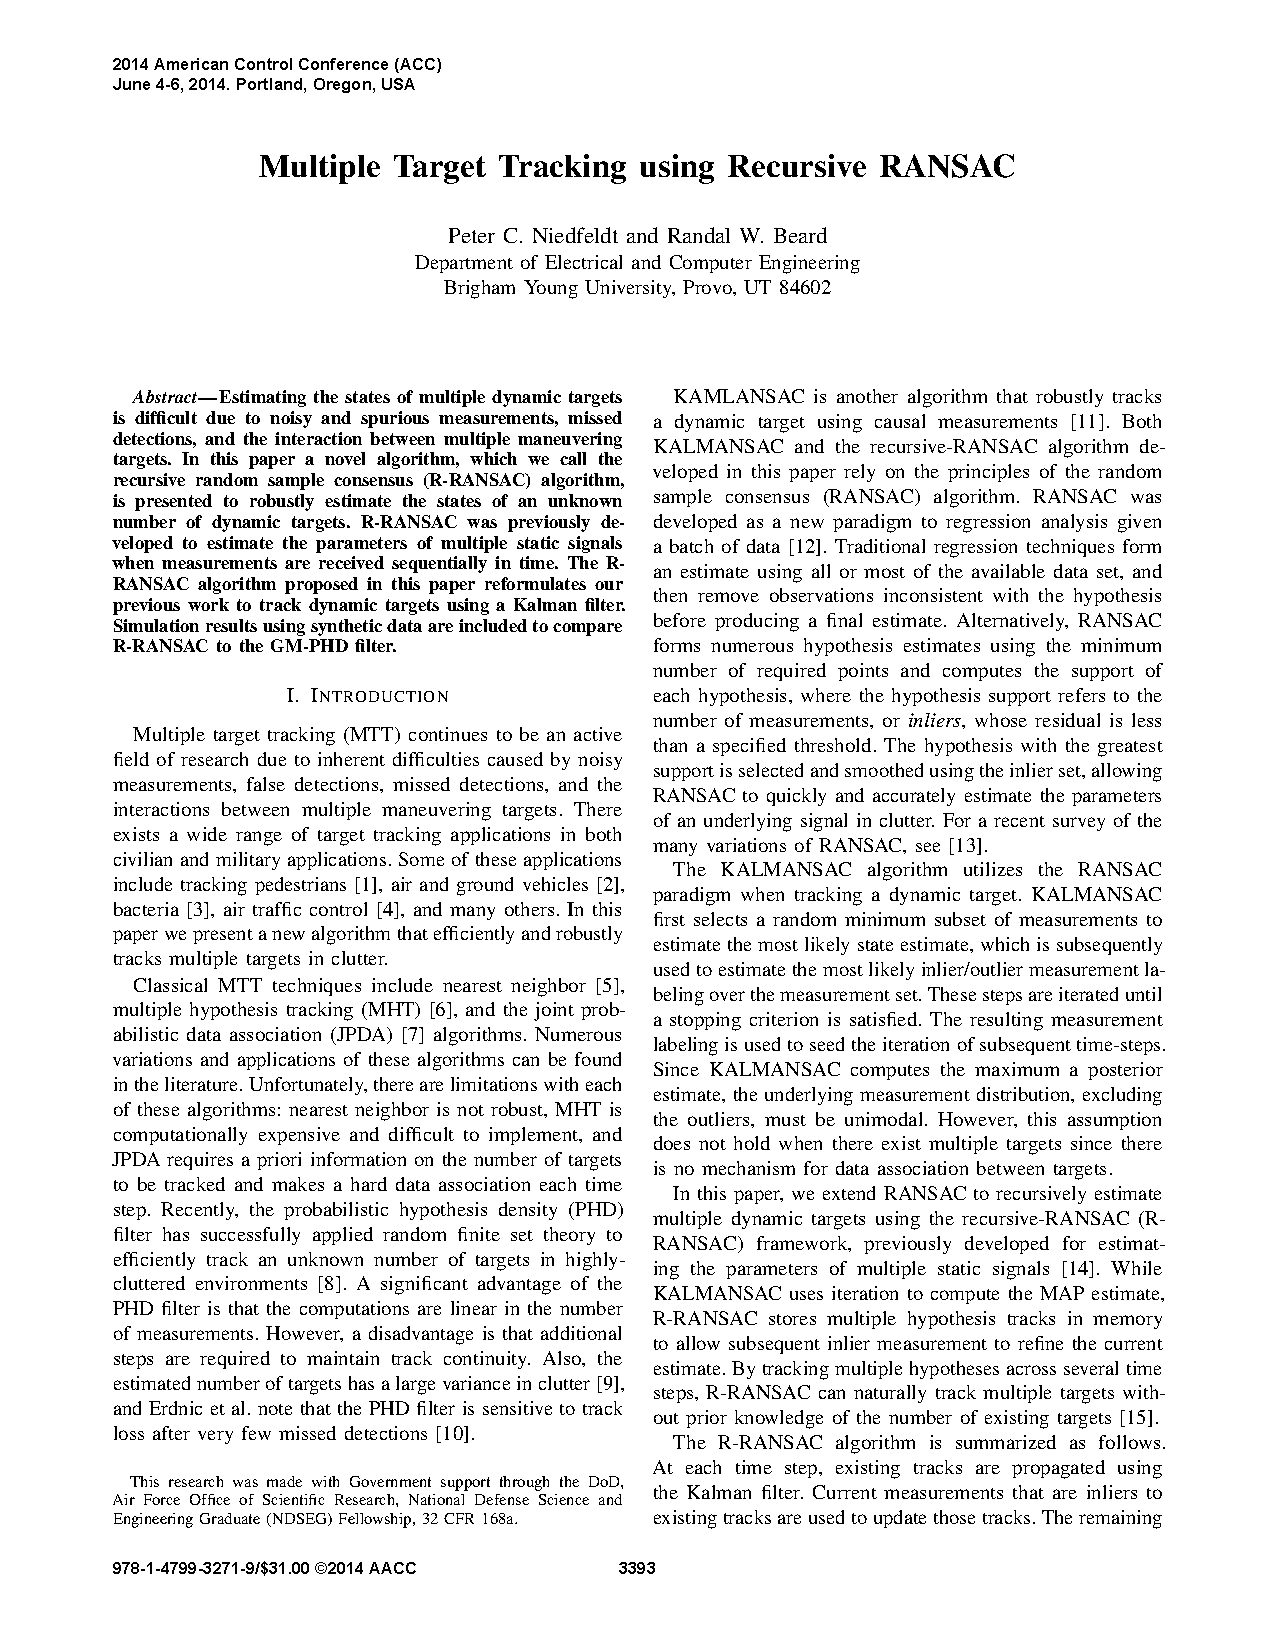
\includepdf[pages=-,scale=.8,pagecommand={}]{chap10_tracking/papers/NiedfeldtBeard14.pdf}


%----------------------------------------------------------------------------
\section{Track Selection}
\label{sec:track_selection}

The R-RANSAC multiple target tracking algorithm returns a set of track, together with covariance information.  One of these tracks needs to be selected to follow.  In the following, we list several posssible options for target following.

%++++++++++++++++
\subsection{Target closest to the image center}
One option is to follow the track that is closest to the image center.  If visual-MTT returns a set of normalized pixel coordinates $\epsilonbf_i$ for the tracks, then select the track that minimizes $\norm{\epsilonbf_i}$.

%++++++++++++++++
\subsection{Template matching}
Suppose that we have a template image of the target that we desire to follow.  The idea is to do a template match located at each potential track.
\sidenote{The \texttt{openCV} function \texttt{matchTemplate} can be used for template matching.}
The template image will be of a certain size and rotation.  Unfortunately, the \texttt{openCV} function \texttt{matchTemplate} is not scale and rotation invariant.  Therefore, given a track location $\epsilonbf_i$, extract a set of scaled and rotated image blocks centered at $\epsilonbf_i$.  The template is then compared to each of these scaled and rotated images, and the best score is assigned to that track.  The track with the best overall score is selected as the track to follow.

A variation of this scheme is when the template, is actually a set of templates, and the scaled and rotated windows from the image are compared to each member of the set.  As the target is followed, additional images of the target can be added to the set of templates to facilitate future tracking.  

Template matching does not need to be performed at each time step, but only at initialization, or when tracks are lost.

%++++++++++++++++
\subsection{Machine learning}
A variation of template matching is to use a machine learning algorithm to identify the track that best matches a learned model.  As with template matching, scale and translation invariance needs to be insured.

%++++++++++++++++
\subsection{User input}
A final method for track selection is to query a user about which track should be followed.  After the user has been queried, templates of the track can be stored in memory, and template matching can be used for continued tracking.


%----------------------------------------------------------------------------
\section{Target following}
\label{sec:target_following}

The tracking problem is best formulated in the body-level frame, as discussed in Section~\ref{sec:body_level_frame}.  

\begin{marginfigure}
	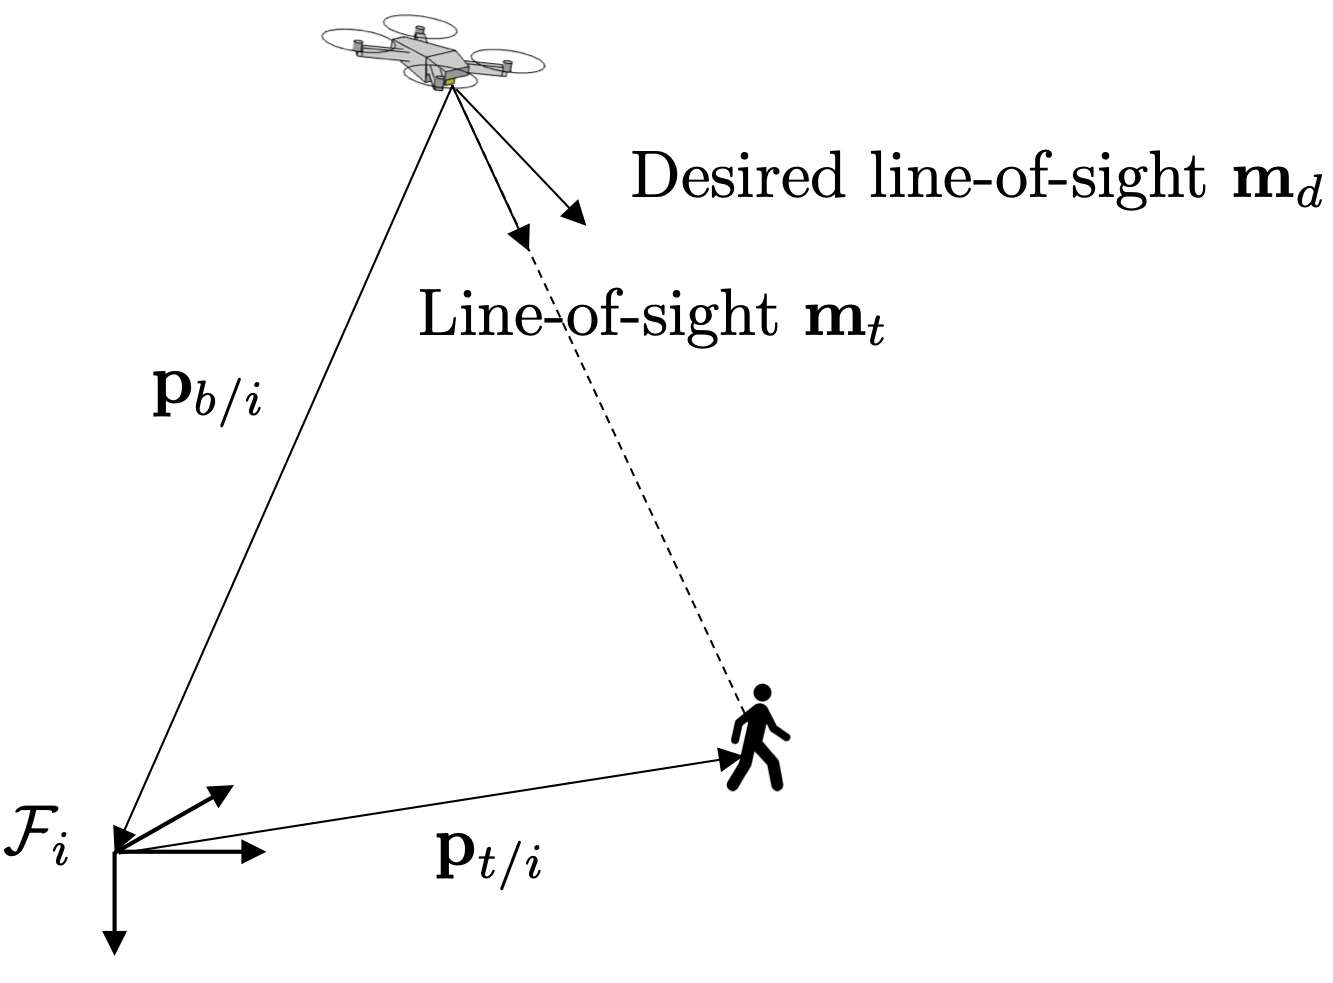
\includegraphics[width=\linewidth]{chap10_tracking/figures/target_following}
	\caption{Definitions and geometry for target following.}
	\label{fig:following}
\end{marginfigure}


Recall that in the body-level frame, the kinematics are given simply as
\[
\dot{\pbf}_{\ell/i}^i = \vbf_{b/i}^i,
\]
where $\vbf_{b/i}^i$ is considered as the input signal to the velocity controller, in addition to the heading vector $\sbf_{\psi} = R_\ell^i \ebf_1$.  

For the target following problem, we will assume that the position of the target in the inertial frame is given by $\pbf_{t/i}^i$, with velocity $\vbf_{t/i}^i$.  The objective is to follow the target at some desired stand-off vector $\pbf_{d/\ell}^\ell$.  
We will assume that the desired stand-off vector $\pbf_{d/\ell}^\ell$ is constant in the level frame.  For example, if the camera is fixed in the body frame, and is oriented so that it points down from the nose with an elevation angle of $-\alpha_0$~degrees, then a stand-off vector of
\[
\pbf_{d/\ell}^\ell = D\begin{pmatrix} \cos\alpha_0 \\ 0 \\ \sin\alpha_0 \end{pmatrix}
\]
is equivalent to commanding the multirotor to follow the target from a slant-range of length $D$.  When perfect tracking is achieved, the set of all possible positions for the multirotor would form a cone about the target with side length $D$.


Let the relative position of the target to the multirotor is given by
\[
\pbf_{t/\ell}^\ell = R_i^\ell \pbf_{t/i}^i - R_i^\ell \pbf_{\ell/i}^i.
\]
The control objective is to maneuver the vehicle so that
\begin{equation}\label{eq:tracking_error}
\pbf_{d/t}^\ell \defeq \pbf_{d/\ell}^\ell - \pbf_{t/\ell}^\ell
\end{equation}
approaches zero asymptotically, or is ultimately uniformly bounded.

Differentiating Equation~\eqref{eq:tracking_error} gives
\begin{align*}
\dot{\pbf}_{d/t}^\ell &= \dot{\pbf}_{d/\ell}^\ell - \dot{\pbf}_{t/\ell}^\ell \\
					  &= - \dot{\pbf}_{t/\ell}^\ell \\
					  &= \vbf_{\ell/i}^\ell - \vbf_{t/i}^\ell \\
					  &= \vbf_{b/i}^\ell - \vbf_{t/i}^\ell,
\end{align*}
where have used the fact that $\pbf_{d/\ell}^\ell$ is constant, and the fact that the position and velocity of the body and body-level frame are identical. 

If the target velocity in the body-level frame is known, and if $\pbf_{t/\ell}^\ell$ can be estimated, then the appropriate body velocity would be
\begin{equation} \label{eq:tracking_body_velocity}
\vbf_{b/i}^\ell = \vbf_{t/i}^\ell - K(\pbf_{d/\ell}^\ell - \pbf_{t/\ell}^\ell),
\end{equation}
where $K=K^\top>0$ so that $\dot{\pbf}_{d/t}^\ell = -k\pbf_{d/t}^\ell$ implies that $\pbf_{d/t}^\ell(t)\to 0$.  

Suppose that the pixel center of the object begin tracked is transformed to the body-level frame according to Lemma~\ref{lem:pixels_in_level_frame}, and is given by $\bar{\epsilon}_{t/\ell}^\ell$, then 
\[
\pbf_{t/\ell}^\ell = \lambda \bar{\epsilon}_{t/\ell}^\ell.
\]
Suppose that the size $S$ of the object being tracked is known, and that the (calibrated) size in the image $\epsilonbf_S$ can be estimated using image processing techniques, then from similar triangles we have $S/lambda = \epsilon_S/1$, or 
\[
\lambda = \frac{S}{\epsilon_S}.
\]
Therefore $\pbf_{t/\ell}^\ell$ can be estimated from image data.  If the target velocity is not known, or cannot be estimated, then implement
\begin{equation}\label{eq:target_following_velocity}
\vbf_{b/i}^i = - R_\ell^i K(\pbf_{d/\ell}^\ell - \frac{S}{\epsilon_S}\bar{\epsilon}_{t/\ell}^\ell).
\end{equation}

The orientation $\sbf_\psi$ is currently a free variable, and we could think of different schemes to select the orientation.  If the objective is to do a tail-chase, then $\sbf_\psi$ should be selected to align with the target velocity $\vbf_{t/i}^i$. 

If $\vbf_{t/i}^i$ is known, then $\sbf_\psi$ can be selected by projecting $\vbf_{t/i}^i$ on to the North-East plane as $\Pi_{\ebf_3}\vbf_{t/i}^i$ and then normalizing to obtain
\begin{equation}\label{eq:tracking_heading_vector}
\sbf_{\psi} = \frac{\Pi_{\ebf_3}\vbf_{t/i}^i}{\norm{\Pi_{\ebf_3}\vbf_{t/i}^i}}.
\end{equation}
\marginnote{Recall that $\Pi_\xbf = I-\xbf\xbf^\top$.  If $\xbf$ is a unit vector, the $\Pi_\xbf$ is a projection matrix on to the plane orthogonal to $\xbf$.}

If $\vbf_{t/i}^i$ is not known, then it can be approximated from image data as follows.  When $\vbf_{b/i}^i$ is selected as in Equation~\eqref{eq:target_following_velocity} then
\[
\dot{\pbf}_{d/t}^i = -R_\ell^i K (\pbf_{d/\ell}^\ell - \pbf_{t/\ell}^\ell) - \vbf_{t/i}^i.
\]
Therefore,
\begin{align*}
\vbf_{t/i}^i &= -R_\ell^i K (\pbf_{d/\ell}^\ell - \pbf_{t/\ell}^\ell) - \dot{\pbf}_{d/t}^i \\
	&= -R_\ell^i \left[ K (\pbf_{d/\ell}^\ell - \frac{S}{\epsilon_S}\bar{\epsilon}_{t/\ell}^\ell) - (\dot{\pbf}_{d/\ell}^\ell - \dot{\lambda}\bar{\epsilonbf}_{t/\ell}^\ell - \lambda\dot{\bar{\epsilonbf}}_{t/\ell}^\ell) \right] \\
	&= -R_\ell^i \left[ K (\pbf_{d/\ell}^\ell - \frac{S}{\epsilon_S}\bar{\epsilon}_{t/\ell}^\ell)  - \frac{S\dot{\epsilon}_S}{\epsilon_S^2}\bar{\epsilonbf}_{t/\ell}^\ell + \frac{S}{\epsilon_S}\dot{\bar{\epsilonbf}}_{t/\ell}^\ell) \right].
\end{align*}
The heading vector is then selected using Equation~\eqref{eq:tracking_heading_vector}.


%----------------------------------------------------------------------------
\section{Target following 2.0}
\label{sec:target_following_2}

The tracking problem is best formulated in the body-level frame, as discussed in Section~\ref{sec:body_level_frame}.  

\begin{marginfigure}
	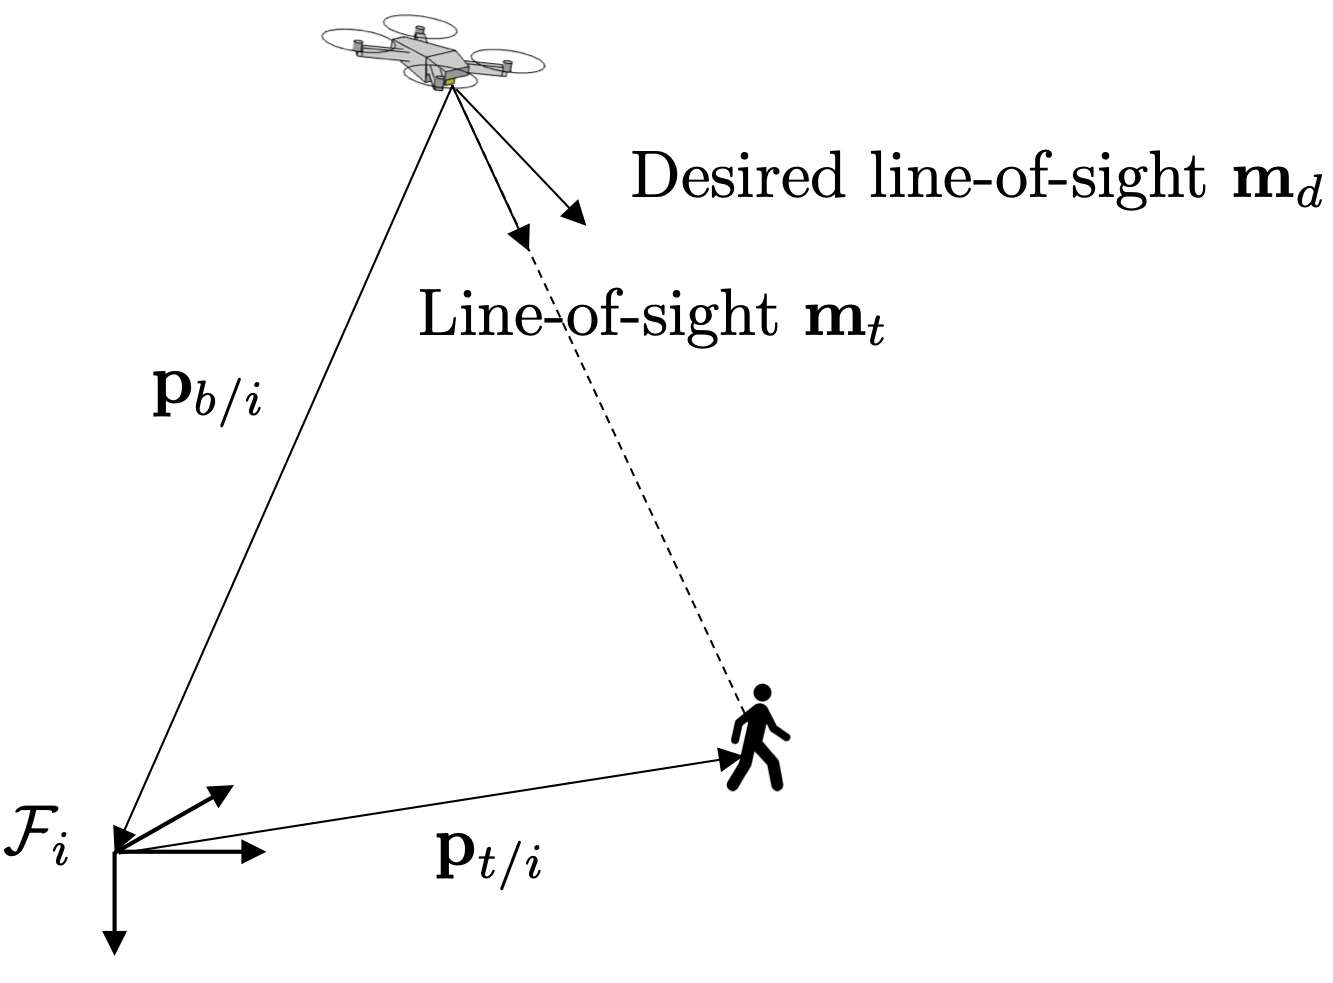
\includegraphics[width=\linewidth]{chap10_tracking/figures/target_following}
	\caption{Definitions and geometry for target following.}
	\label{fig:following}
\end{marginfigure}

Recall that in the body-level frame, the kinematics are given simply as
\begin{equation}\label{eq:multirotor_tracking_eom}
\dot{\pbf}_{\ell/i}^i = \vbf_{b/i}^i,
\end{equation}
where $\vbf_{b/i}^i$ is considered as the input signal to the velocity controller, in addition to the heading vector $\sbf_{\psi} = R_\ell^i \ebf_1$.  

The normalized line-of-sight vector between the multirotor and the target is given by
\[
\mbf_t \defeq \frac{\pbf_{t/i} - \pbf_{b/i}}{\norm{\pbf_{t/i} - \pbf_{b/i}}}.
\]
Note that the normalized line of sight vector can be computed from the calibrated pixel coorinates as 
\[
\mbf_t = \frac{\epsilonbf_t}{\norm{\epsilonbf_t}}.
\]
Recall from Property~\ref{prop:derivative_of_normal_vector} that 
\begin{align}
\frac{d\mbf_t}{dt} &= \Pi_{\mbf_t} \frac{\dot{\pbf}_{t/i} - \dot{\pbf}_{b/i}}{\norm{\pbf_{t/i} - \pbf_{b/i}}} \notag \\
	&= \Pi_{\mbf_t} \frac{\dot{\pbf}_{t/i} - \vbf_{b/i}}{\norm{\pbf_{t/i} - \pbf_{b/i}}}, \label{eq:mbf_t_dot}
\end{align}
where $\Pi_\nbf = I-\nbf\nbf^\top$ is the projection operator onto the plane orthogonal to the normal vector $\nbf$.  


The tracking objective is to maneuver the multirotor so that the normalized line-of-sight vector $\mbf_t$ is equal to a desired normalized line-of-sight vector $\mbf_d$, as shown in Figure~\ref{fig:following}.  For example, if the camera is fixed in the body frame, and is oriented so that it points down from the nose with an elevation angle of $-\alpha_0$~degrees, and the objective is to keep the target in the center of the field of view, then the desired normalized line-of-sight vector would be
\[
\mbf_d = \begin{pmatrix} \cos\alpha_0 \\ 0 \\ \sin\alpha_0 \end{pmatrix}.
\]

\begin{marginfigure}
	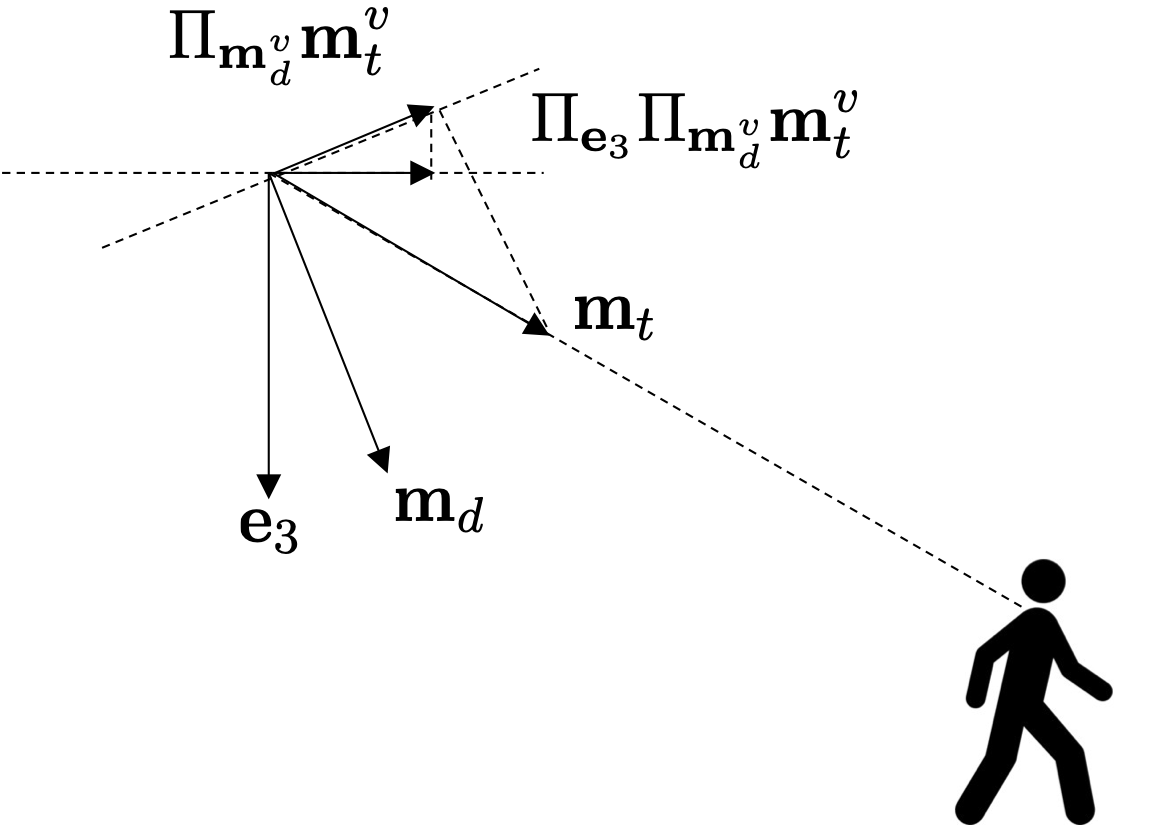
\includegraphics[width=\linewidth]{chap10_tracking/figures/target_following_geometry}
	\caption{target following goemetry}
	\label{fig:target_following_geometry}
\end{marginfigure}
The intuition behind the control law introduced below is illustrated in Figure~\ref{fig:target_following_geometry}.
The error between the line-of-sight vector $\mbf_t$ and the desired line-of-sight vector $\mbf_d$ can be expressed as
\[
\nubf_1 = \Pi_{\mbf_d^v} \mbf_t^v
\]
where $\nubf_1$ is the projection of $\mbf_t$ onto the plane orthogonal to $\mbf_d$.  Note that when $\mbf_t=\mbf_d$, then $\nubf_1=0$.  

We will assume for the moment that the multirotor will only be commanded to perform lateral motion.  Therefore, projecting $\nubf_1$ onto the lateral plane gives the error vector
\[
\nubf = \Pi_{\ebf_3}\Pi_{\mbf_d^v}\mbf_t^v. 
\]
The multirotor velocity is selected to be proportional to this error as 
\begin{equation} \label{eq:multirotor_tracking_velocity}
\vbf_{b/i}^i = k \Pi_{\ebf_3} \Pi_{\mbf_d^v} \mbf_t^v.
\end{equation}

\begin{theorem}
	Suppose that the equations of motion for the multirotor are given in Equation~\eqref{eq:multirotor_tracking_eom}, and that the target velocity satisfies $\vbf_{t/i}^i=0$, and the vehicle velocity is given by Equation~\eqref{eq:multirotor_tracking_velocity}.
	If the altitude of the multi-rotor is greater than the altitude of the target, and if the desired line-of-sight vector points down, i.e., $\ebf_3^\top \mbf_d^v$, 	
	then $\mbf_t(t) \to \mbf_d$.
	
\end{theorem}
\begin{proof}
	Consider the Lyapunov function candidate
	\begin{align*}
		V &= \frac{1}{2} \norm{\mbf_d \times \mbf_t}^2 \\
	  	&= \frac{1}{2} \norm{\ss{\mbf_d} \mbf_t}^2 \\
	  	&= \frac{1}{2} \mbf_t^\top \ss{\mbf_d}^\top \ss{\mbf_d} \mbf_t \\
	  	&= -\frac{1}{2} \mbf_t^\top \ss{\mbf_d}^2 \mbf_t \\ 
	  	&= \frac{1}{2} \mbf_t^\top \Pi_{\mbf_d} \mbf_t,
	\end{align*}
	where we have used the fact that $\ss{\xbf}^2 = \xbf\xbf^\top - \xbf^\top\xbf I$, implying that $\ss{\mbf_d}^2 = -\Pi_{\mbf_d}$.  
	Taking the derivative of $V$ gives
	\begin{align*}
		\dot{V} &= \mbf_t^\top \Pi_{\mbf_d} \dot{\mbf}_t \\
			    &= \mbf_t^\top \Pi_{\mbf_d} \Pi_{\mbf_t} \frac{\dot{\pbf}_{t/i} - \vbf_{b/i}}{\norm{\pbf_{t/i} - \pbf_{b/i}}} \\
			    &= -\mbf_t^\top \Pi_{\mbf_d} \Pi_{\mbf_t} \frac{\vbf_{b/i}}{\norm{\pbf_{t/i} - \pbf_{b/i}}} \\
			    &= -\frac{k}{\norm{\pbf_{t/i} - \pbf_{b/i}}}\mbf_t^\top \Pi_{\mbf_d} \Pi_{\mbf_t} \Pi_{\ebf_3} \Pi_{\mbf_d^v} \mbf_t^v,
	\end{align*}
	where we have used Equations~\eqref{eq:mbf_t_dot} and~\eqref{eq:multirotor_tracking_velocity}.
	Using the definition of $\Pi_\nbf$, after some algebra, we get that
	\begin{align*}
		\dot{V} &=  -\frac{k}{\norm{\pbf_{t/i} - \pbf_{b/i}}} \mbf_t^\top (I-\mbf_d\mbf_d^\top) (I-\mbf_t\mbf_t^\top) (I-\ebf_3\ebf_3^\top) (I-\mbf_d\mbf_d^\top)  \mbf_t^v, \\
				&= -\frac{k}{\norm{\pbf_{t/i} - \pbf_{b/i}}} (1-(\mbf_t^\top\mbf_d)^2)(\mbf_t^\top \mbf_d)(1+(\ebf_3^\top \mbf_t)(\ebf_3^\top \mbf_d)).  
	\end{align*}
	If the altitude of the multirotor is greater than the altitude of the target, then $\ebf_3^\top \mbf_t > 0$.   In addition, since both $\mbf_t$ and $\mbf_d$ point down, we have that $\mbf_t^\top \mbf_d > 0$.  And since $\mbf_t$ and $\mbf_d$ are both unit vectors, Cauchy's inequality gives that $(\mbf_t^\top \mbf_d)^2 \leq 1$ where equality hold only when $\mbf_t=\mbf_d$.  Therefore $\dot{V}$ is negative definite, implying that $\mbf_t \to \mbf_d$.  
	
\end{proof}



The orientation $\sbf_\psi$ is currently a free variable, and we could think of different schemes to select the orientation.  If the objective is to do a tail-chase, then $\sbf_\psi$ should be selected to align with the target velocity $\vbf_{t/i}^i$. 

If $\vbf_{t/i}^i$ is known, then $\sbf_\psi$ can be selected by projecting $\vbf_{t/i}^i$ on to the North-East plane as $\Pi_{\ebf_3}\vbf_{t/i}^i$ and then normalizing to obtain
\begin{equation}\label{eq:tracking_heading_vector}
\sbf_{\psi} = \frac{\Pi_{\ebf_3}\vbf_{t/i}^i}{\norm{\Pi_{\ebf_3}\vbf_{t/i}^i}}.
\end{equation}
\marginnote{Recall that $\Pi_\xbf = I-\xbf\xbf^\top$.  If $\xbf$ is a unit vector, the $\Pi_\xbf$ is a projection matrix on to the plane orthogonal to $\xbf$.}



%----------------------------------------------------------------------------
\section{Autonomous Flight for Detection, Localization, and Tracking of Moving Targets with Small Quadrotor, RA-L, 2017 (in review)}
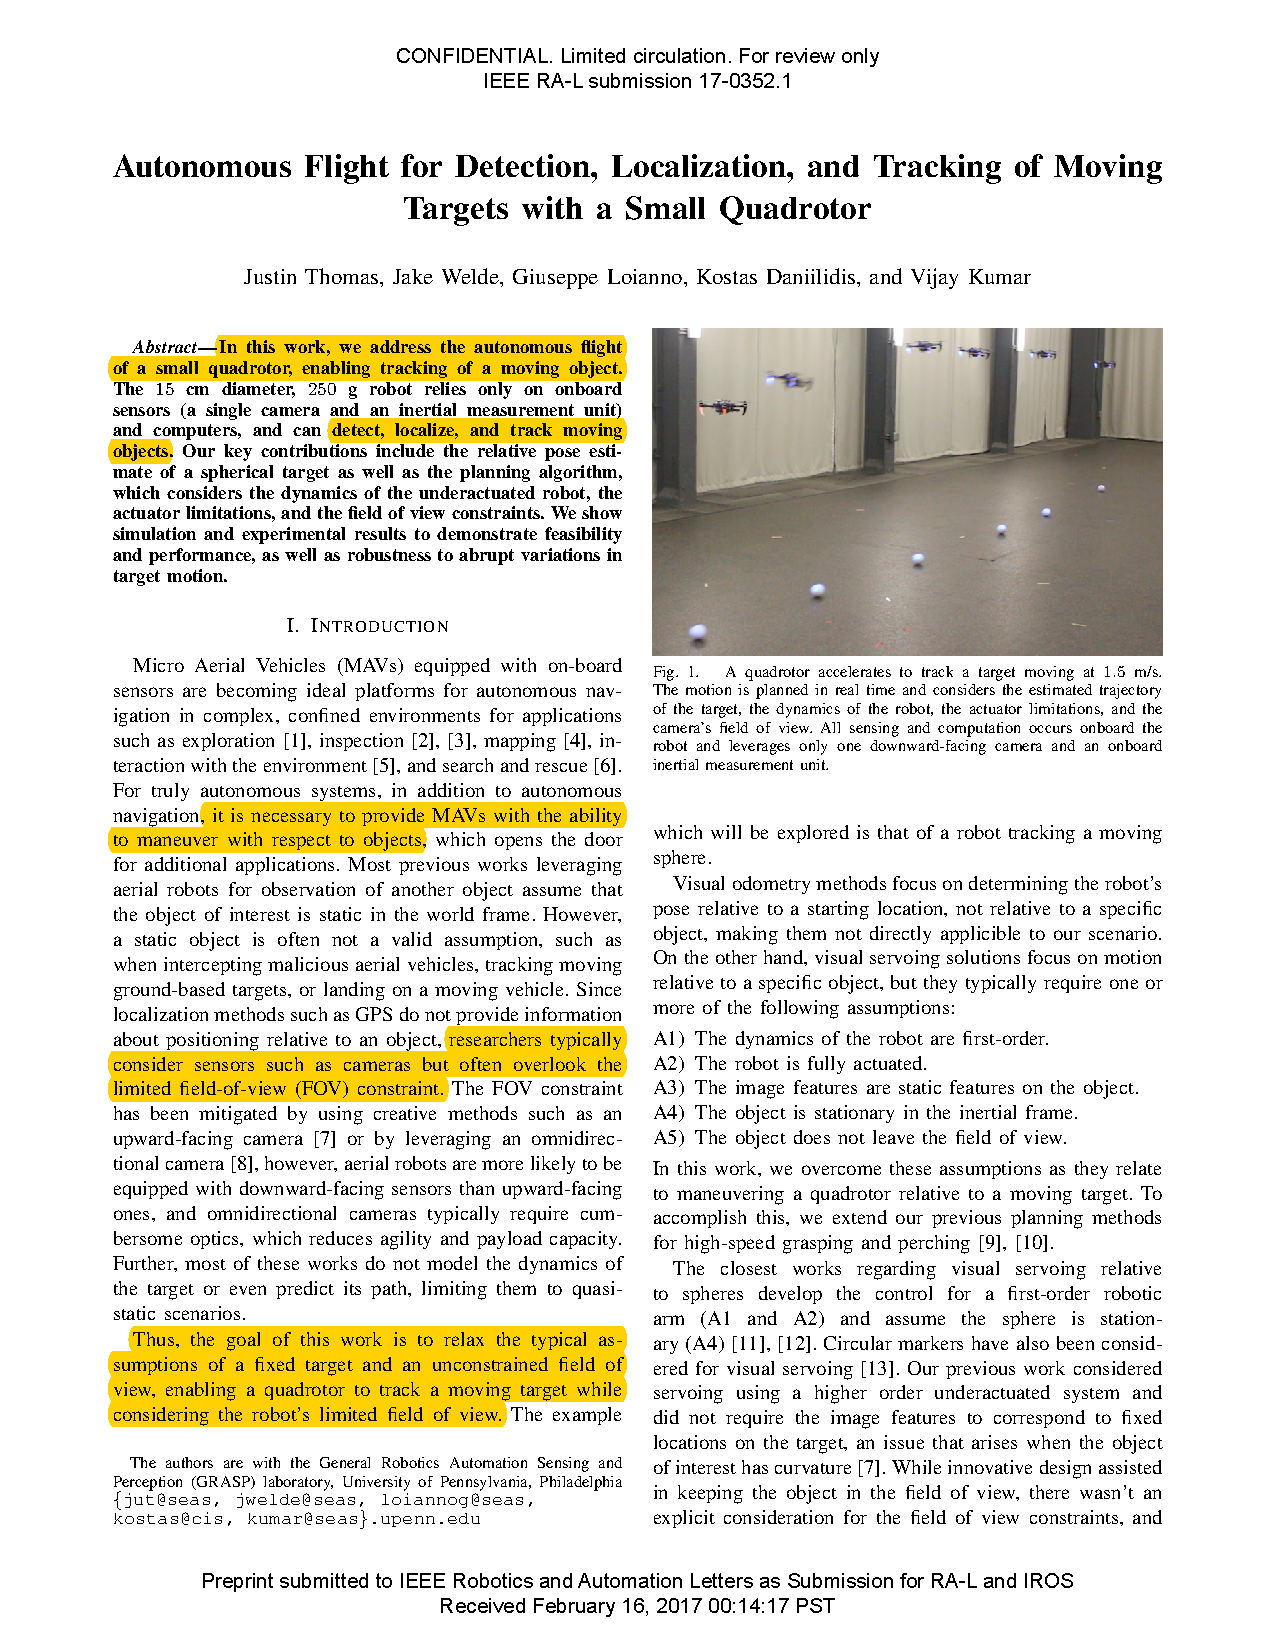
\includepdf[pages=-,scale=.8,pagecommand={}]{chap10_tracking/papers/ThomasWeldeLoianno16.pdf}



